\documentclass[12pt,a4paper]{report}

\usepackage[utf8]{inputenc}
\usepackage[spanish]{babel}
\usepackage{graphicx}
\usepackage{amsmath}
\usepackage{amssymb}
\usepackage{hyperref}
\usepackage{comment}
\usepackage{geometry}
\usepackage{caption}
\usepackage{subcaption}

\geometry{a4paper, margin=1in}

\title{Detección Multimodal de Animales para el Ciber-Pastoreo de Ganado}
\author{
    Jorge Urbón Burgos \\
    \texttt{777295@unizar.es}
    \and
    Supervisor: Rosario Aragües \\
    \texttt{raragues@unizar.es}
    \and
    Co-Supervisor: Jesús Bermúdez \\
    \texttt{bermudez@unizar.es}
}
\date{\today}

\begin{document}

\maketitle

\begin{abstract}
% TODO: add abstract
\end{abstract}

\tableofcontents

\chapter{Introducción}
\label{chap:introduction}

\section{Motivación}
\label{sec:motivation}
Este trabajo parte a raíz de lo propuesto en el proyecto \texttt{COUNTRYBOTS} llevado a cabo por el grupo \texttt{Ropert}, cuyo principal objetivo es la automatización y robotización de tareas agrícolas y ganaderas mediante el uso de sistemas multirobot que combinan imágenes aéreas para una mejor monitorización del entorno.

La motivación del trabajo aquí presentado radica en la necesidad de diferentes barreras que la monitorización de animales puede presentar, siendo el \textit{trackeo} de animales mediante el uso de varias modalidades una posible solución a estos problemas. La segmentación multimodal en visión artificial tiene el potencial de mejorar significativamente el desempeño de las labores de ciber-pastoreo y vigilancia de animales en entornos naturales, ya que la información adicional que diferentes modalidades (o las interacciones entre las mismas) puede aportar al modelo puede ser clave para la correcta segmentación de los animales en la escena.

Este trabajo se centra principalmente en explorar, implementar y evaluar diferentes técnicas multimodales para el \textit{trackeo} de animales.

\section{Objetivos}
\label{sec:objectives}
El objetivo de este trabajo es, por tanto, la verificación de la utilidad de las técnicas multimodales para la identificación y monitoreo de animales en entornos naturales con el fin de demostrar su utilidad de cara a conseguir característica más ricas y completas. Para ello, se analizarán diferentes técnicas basadas en \textit{Deep Learning} y se evaluarán los resultados obtenidos.

\section{Trabajos Relacionados}
\label{sec:related_work}
El campo de la visión por computador ha sufrido una enorme revolución a lo largo de la última década gracias, principalmente, a los avances en \textit{Deep Learning}. A continuación se presentan algunos de los trabajos más relevantes en lo referente a este trabajo.

\subsection{Redes Convolucionales}
\label{subsec:cnn}
A pesar de la antigüedad del concepto, las redes neuronales convolucionales \texttt{CNN} supusieron un gran avance en el reconocimiento de imagenes desde la introducción de \texttt{AlexNet} en \cite{NIPS2012_c399862d}. Desde entonces, las \texttt{CNN} han sido ampliamente utilizadas una gran variedad de tareas relacionadas con la Visión por Computador como la clasificación de imágenes, detección y segmentación de objetos. A lo largo de este trabajo, se emplearán diferentes técnicas que ponen en uso este tipo de redes neuronales.

\subsection{UNets}
\label{subsec:unets}
Los modelos \texttt{UNet}, presentados originalmente en \cite{ronneberger2015unetconvolutionalnetworksbiomedical} como una alternativa para la segmentación de imágenes biomédicas, han sido ampliamente utilizados en tareas de segmentación generales debido a su arquitectura sencilla y efectiva consistente en una serie de bloques de \textit{upsampling} y \textit{downsampling} que permiten al modelo aprender características a diferentes niveles de abstracción en la imagen de entrada (mostrado en la figura \ref{fig:unet-architecture}). Este tipo de modelos, aunque relativamente antiguos, siguen siendo relevantes en la actualidad e incluso se han llegado a implementar versiones multimodales como \cite{huang2024mmaunetmultimodalasymmetricunet} o \cite{marinov2023mirrorunetmarryingmultimodal}.

\begin{figure}[!h]
    \centering
    \includegraphics[width=0.5\textwidth]{media/model/unet.png}
    \caption{Arquitectura de un modelo \texttt{UNet}}
    \label{fig:unet-architecture}
\end{figure}

\subsection{Mask R-CNN}
\label{subsec:maskrcnn}
Como sucesor a \texttt{Faster R-CNN} (trabajo presentado en \cite{girshick2015fastrcnn} que se limita a la detección de regiones de interés \texttt{RoI}), \texttt{Mask R-CNN} (\cite{he2018maskrcnn}) se presenta como una amplia mejora de su predecesor al incluir una rama de segmentación de instancias en paralelo a la rama de detección de objetos como se muestra en la figura \ref{fig:mask-rcnn-architecture}

\begin{figure}[!h]
    \centering
    \includegraphics[width=0.5\textwidth]{media/model/mask_rcnn.png}
    \caption{Arquitectura de un modelo \texttt{Mask R-CNN}}
    \label{fig:mask-rcnn-architecture}
\end{figure}

\subsection{Transformers}
\label{subsec:transformers}
Uno de los más recientes y posiblemente más relevantes avances en el campo del \textit{Deep Learning} ha sido la introducción de los modelos \texttt{Transformers} en \cite{vaswani2023attentionneed}. Estos modelos han sido amplia y popularmente empleados en tareas de procesamiento de lenguaje natural (\texttt{NLP}) en los últimos años(\cite{radford2018improving}, \cite{devlin2019bertpretrainingdeepbidirectional}, \cite{raffel2023exploringlimitstransferlearning}) debido a la ya demostrada eficacia de su arquitectura basada en la \textit{self attention}, aunque también han supuesto un gran progreso en las tareas de visión por computador tras la demostración en \cite{dosovitskiy2021imageworth16x16words} de que pueden incluso superar el rendimiento de las \texttt{CNN} en tareas de clasificación.

% \begin{figure}[!h]
%     \centering
%     \includegraphics[width=0.5\textwidth]{media/model/transformer_architecture.png}
%     \caption{Arquitectura base de un modelo \texttt{Transformer}}
%     \label{fig:transformer-architecture}
% \end{figure}

La capacidad de este tipo de arquitecturas en tareas de segmentación ya ha sido demostrada en una variedad de trabajos (\cite{carion2020endtoendobjectdetectiontransformers}, \cite{xie2021segformersimpleefficientdesign}, \cite{strudel2021segmentertransformersemanticsegmentation}) y se espera que su aplicación en tareas multimodales como la segmentación de imágenes sea igualmente efectiva.

\subsection{Monitorización de Animales}
\label{subsec:animal_monitoring}
Aunque no se trate de un tema tan ampliamente estudiado como la segmentación de imágenes, la monitorización de animales también se ha visto beneficiada por los avances en visión por computador dados en los últimos años. Proyectos como \cite{sheepcounter-odziz_dataset}, \cite{birdsai-duqdg_dataset}, \cite{guillen-garde_detection_2021} o estudios del arte como \cite{XU2024103732} demuestran ya la utilidad técnicas de localización de animales basadas en \textit{deep learning} mediante el uso de imágenes aéreas. 

\chapter{Datos}
\label{chap:data}
Dado el objetivo que se tiene en este trabajo de verificar la utilidad de las técnicas de segmentación multimodales en la identificación y segmentación de animales en imágenes en entornos naturals, se focaliza la búsqueda en \textit{datasets} que contengan, idealmente, parejas de imágenes multimodales que ya hayan sido sincronizadas, alineadas y etiquetadas previamente con el fin de facilitar el proceso de entrenamiento y validación de los modelos. Además, se busca que dichos posibles \textit{datasets} contengan una variedad de animales y situaciones que permitan una generalización adecuada de los modelos a entrenar.

\section{Datasets Disponibles}
\label{sec:available_datasets}
Con el fin de encontrar un conjunto de datos que se adecúe a las necesidades anteriormente expresadas, se realiza una búsqueda exhaustiva de \textit{datasets} disponibles de forma pública en internet. Cabe destacar las particularidades bajo las que se trabaja, ya que no solo se requiere que el \textit{dataset} contenga imágenes de animales, si no que además se necesita que más de una modalidad esté presente y que los datos hayan sido ya etiquetados y estén listos para el entrenamiento. A continuación, se presentan estos \textit{datasets} y se analizan sus características.

\textbf{NOAA Arctic Seals 2019}: este \textit{dataset} presentado en \cite{noaa_alaska_fisheries_2021} cuenta con alrededor de 80.000 pares de imágenes a color (\texttt{RGB}) e infrarojas térmicas (\texttt{IRT}) tomadas desde el aire durante vuelos desarrollados en Alaska. A pesar de que este \textit{dataset} cuenta con una gran cantidad de imágenes (incluyendo unas 14.000 \textit{bounding boxes}), la variedad de animales presentes en el mismo es limitada, por lo que no se considera adecuado para este trabajo.

\textbf{UAV-derived waterfowl thermal imagery dataset}: este \textit{dataset} presentado en \cite{uav_waterfowl_thermal_2021} también consiste en imágenes aéreas de aves acuáticas tomadas con cámaras infrarojas térmicas (\texttt{IRT}) y cámaras \texttt{RGB} desde un \textit{drone} sobre la región de Nebraska. El \textit{dataset} cuenta con 8.976 \textit{bounding boxes}, sin embargo sus modalidades no se encuentran alineadas, lo que dificultaría mucho el proceso de entrenamiento de los modelos.

\textbf{Lindenthal Camera Traps}: este otro \textit{dataset} presentado en \cite{haucke2021exploitingdepthinformationwildlife} está construido a partir de pares infrarojos para visión nocturna (\texttt{IR}) y mapas de profundidad (\texttt{D}) obtenidos a través de una cámara estéreo fija a pocos metros del suelo. Este dataset cuenta con un total de 1.038 instancias segmentadas de animales de 4 clases diferenciadas. A pesar de que este \textit{dataset} cuenta con una cantidad de imágenes mucho menor que los anteriores, la calidad de las imágenes y la variedad en el tipo de animales presentes en el mismo lo hacen ideal para este trabajo.

\section{Lindenthal Camera Traps Dataset}
\label{sec:lindenthal_dataset}
De entre los \textit{datasets} públicos disponibles, el más completo y adecuado para este propósito se trata de \texttt{Lindenthal Camera Traps} presentado por \cite{haucke2021exploitingdepthinformationwildlife}, por lo que durante este proyecto se empleará una parte\footnote{A pesar de que este \textit{dataset} cuenta con 775 secuencias de video que incluyen información \texttt{RGB} durante el día o \texttt{IR} durante la noche, así como mapas de profundidad en ambos casos, tan solo fueron etiquetados para su uso como \textit{Ground Truth} 12 videos nocturnos, de los cuales se etiqueraría cada décimo fotograma.} del mismo. Este \textit{dataset} está constituido por imágenes de animales en el Zoo de Lindenthal, Colonia, obtenidas con una cámara estéreo \texttt{Intel RealSense D435} y en el que se incluyen imágenes infrarojas (\texttt{IR}) con una profundidad de 8 bits y mapas de profundidad (\texttt{D}) con una profundidad de 16 bits en los que el valor de cada pixel representa la distancia en milimetros\footnote{El sensor \texttt{Intel RealSense D435} cuenta con la capacidad de obtener imágenes estéreo de forma activa empleando ambas cámaras infrarojas mediante la proyección de un patrón infrarojo en la escena, sin embargo al haberse construido este dataset a partir de imagenes nocturnas en las que dicho patrón sería visible al sensor \texttt{IR}, se optó por generar los mapas de profundidad \texttt{D} mediante el uso de la cámara estéreo en modo pasivo.}. Ambas modalidades se encuentran ya alineadas y sincronizadas, lo que permite un fácil acceso a la información de ambas modalidades. Además, el etiquetado de los animales se encuentra en formato \texttt{COCO}. En la figura \ref{fig:base-data-lindenthal} se muestra un ejemplo de una pareja de imágenes \texttt{IR} y \texttt{D} del \textit{dataset}. La captura de estas imagenes se realiza desde el tejado de un establo, lo que permite una vista elevada de los animales en la escena. Además, los datos se capturan exclusivamente cuando se da algun tipo de movimiento, por lo que en el \textit{setup} indicado se incluye un sensor infrarojo pasivo (\texttt{PIR}) que actúa como sensor de movimiento.
\begin{figure}[!h]
    \centering
    \begin{subfigure}{0.45\textwidth}
        \centering
        \includegraphics[width=\textwidth]{media/data/ir_gueese.jpg}
        \caption{Imagen \texttt{IR}}
    \end{subfigure}
    \hfill
    \begin{subfigure}{0.45\textwidth}
        \centering
        \includegraphics[width=\textwidth]{media/data/depth_gueese.png}
        \caption{Imagen de profundidad}
    \end{subfigure}
    \caption{Ejemplo de una pareja \texttt{IR}-\texttt{D} del \textit{dataset} \texttt{Lindenthal Camera Traps}}
    \label{fig:base-data-lindenthal}
\end{figure}

\subsection{Desglose del \textit{Dataset}}
El \textit{dataset} consiste en doce videos para los que se ha etiquetado cada décimo fotograma, lo que supone un total de 412 pares \texttt{IR}-\texttt{D} con 1038 instancias etiquetadas en formato \texttt{COCO} que incluyen la máscara, la caja delimitadora de la misma, la categoría y un identificador único para cada uno de los animales. Las categorías de animales presentes en el dataset son \textbf{Deer}, \textbf{Goat}, \textbf{Donkey} y \textbf{Goose}, siendo considerado todo lo demás descartable, es decir, parte de la categoría \textbf{Background}. En la figura \ref{fig:dataset-breakdown} se muestra un desglose de la frecuencia de aparición de cada categoría en el dataset y se puede observar el amplio desbalanceo entre distintas categorías, por lo que cabe esperar que el modelo tenga ciertas dificultades a la hora de segmentar las categorías menos frecuentes como por ejemplo \textbf{Donkey}.
\begin{figure}[!h]
    \centering
    \includegraphics[width=0.5\textwidth]{media/data/dataset_breakdown.png}
    \caption{Desglose de la frecuencia de aparición de cada categoría en el dataset}
    \label{fig:dataset-breakdown}
\end{figure}
Por otra parte, este \textit{dataset} se mezclará aleatoriamente y se dividirá en dos partes: el 85\% de las imágenes se emplearán para entrenamiento y el 15\% restante para validación de los resultados con el fin de aplicar técnicas como el \texttt{EarlyStopping} o simplemente para una verificación manual del buen entrenamiento durante el proceso. En la figura \ref{fig:tagged-example} se muestra un ejemplo de un par \texttt{IR}-\texttt{D} con sus respectivas máscaras de segmentación extraidas del etiquetado \texttt{COCO}.
\begin{figure}[!h]
    \centering
    \begin{subfigure}{0.45\textwidth}
        \centering
        \includegraphics[width=\textwidth]{media/data/mask_gueese_ir.png}
        \caption{Imagen \texttt{IR} etiquetada}
    \end{subfigure}
    \hfill
    \begin{subfigure}{0.45\textwidth}
        \centering
        \includegraphics[width=\textwidth]{media/data/mask_gueese_de.png}
        \caption{Imagen \texttt{D} etiquetada}
    \end{subfigure}
    \caption{Ejemplo de una pareja \texttt{IR}-\texttt{D} del \textit{dataset} \texttt{Lindenthal Camera Traps}}
    \label{fig:tagged-example}
\end{figure}

\chapter{Cross Modal Fusion}
\label{chap:cmx}
\section{Descripción del Modelo}
\label{sec:cmx_description}
El primer modelo a implementar en este trabajo se trata de \texttt{CrossModalFusion} (\texttt{CMX}), presentado por \cite{zhang2023cmxcrossmodalfusionrgbx}. Este modelo propone una arquitectura para la segmentación semántica de pares \texttt{RGB-X} diseñada para aprovechar las características complementarias entre imágenes \texttt{RGB} y diversas modalidades como la térmica, imágenes de eventos o, como es de nuestro interés, imágenes de profundidad.

\begin{figure}[!h]
    \centering
    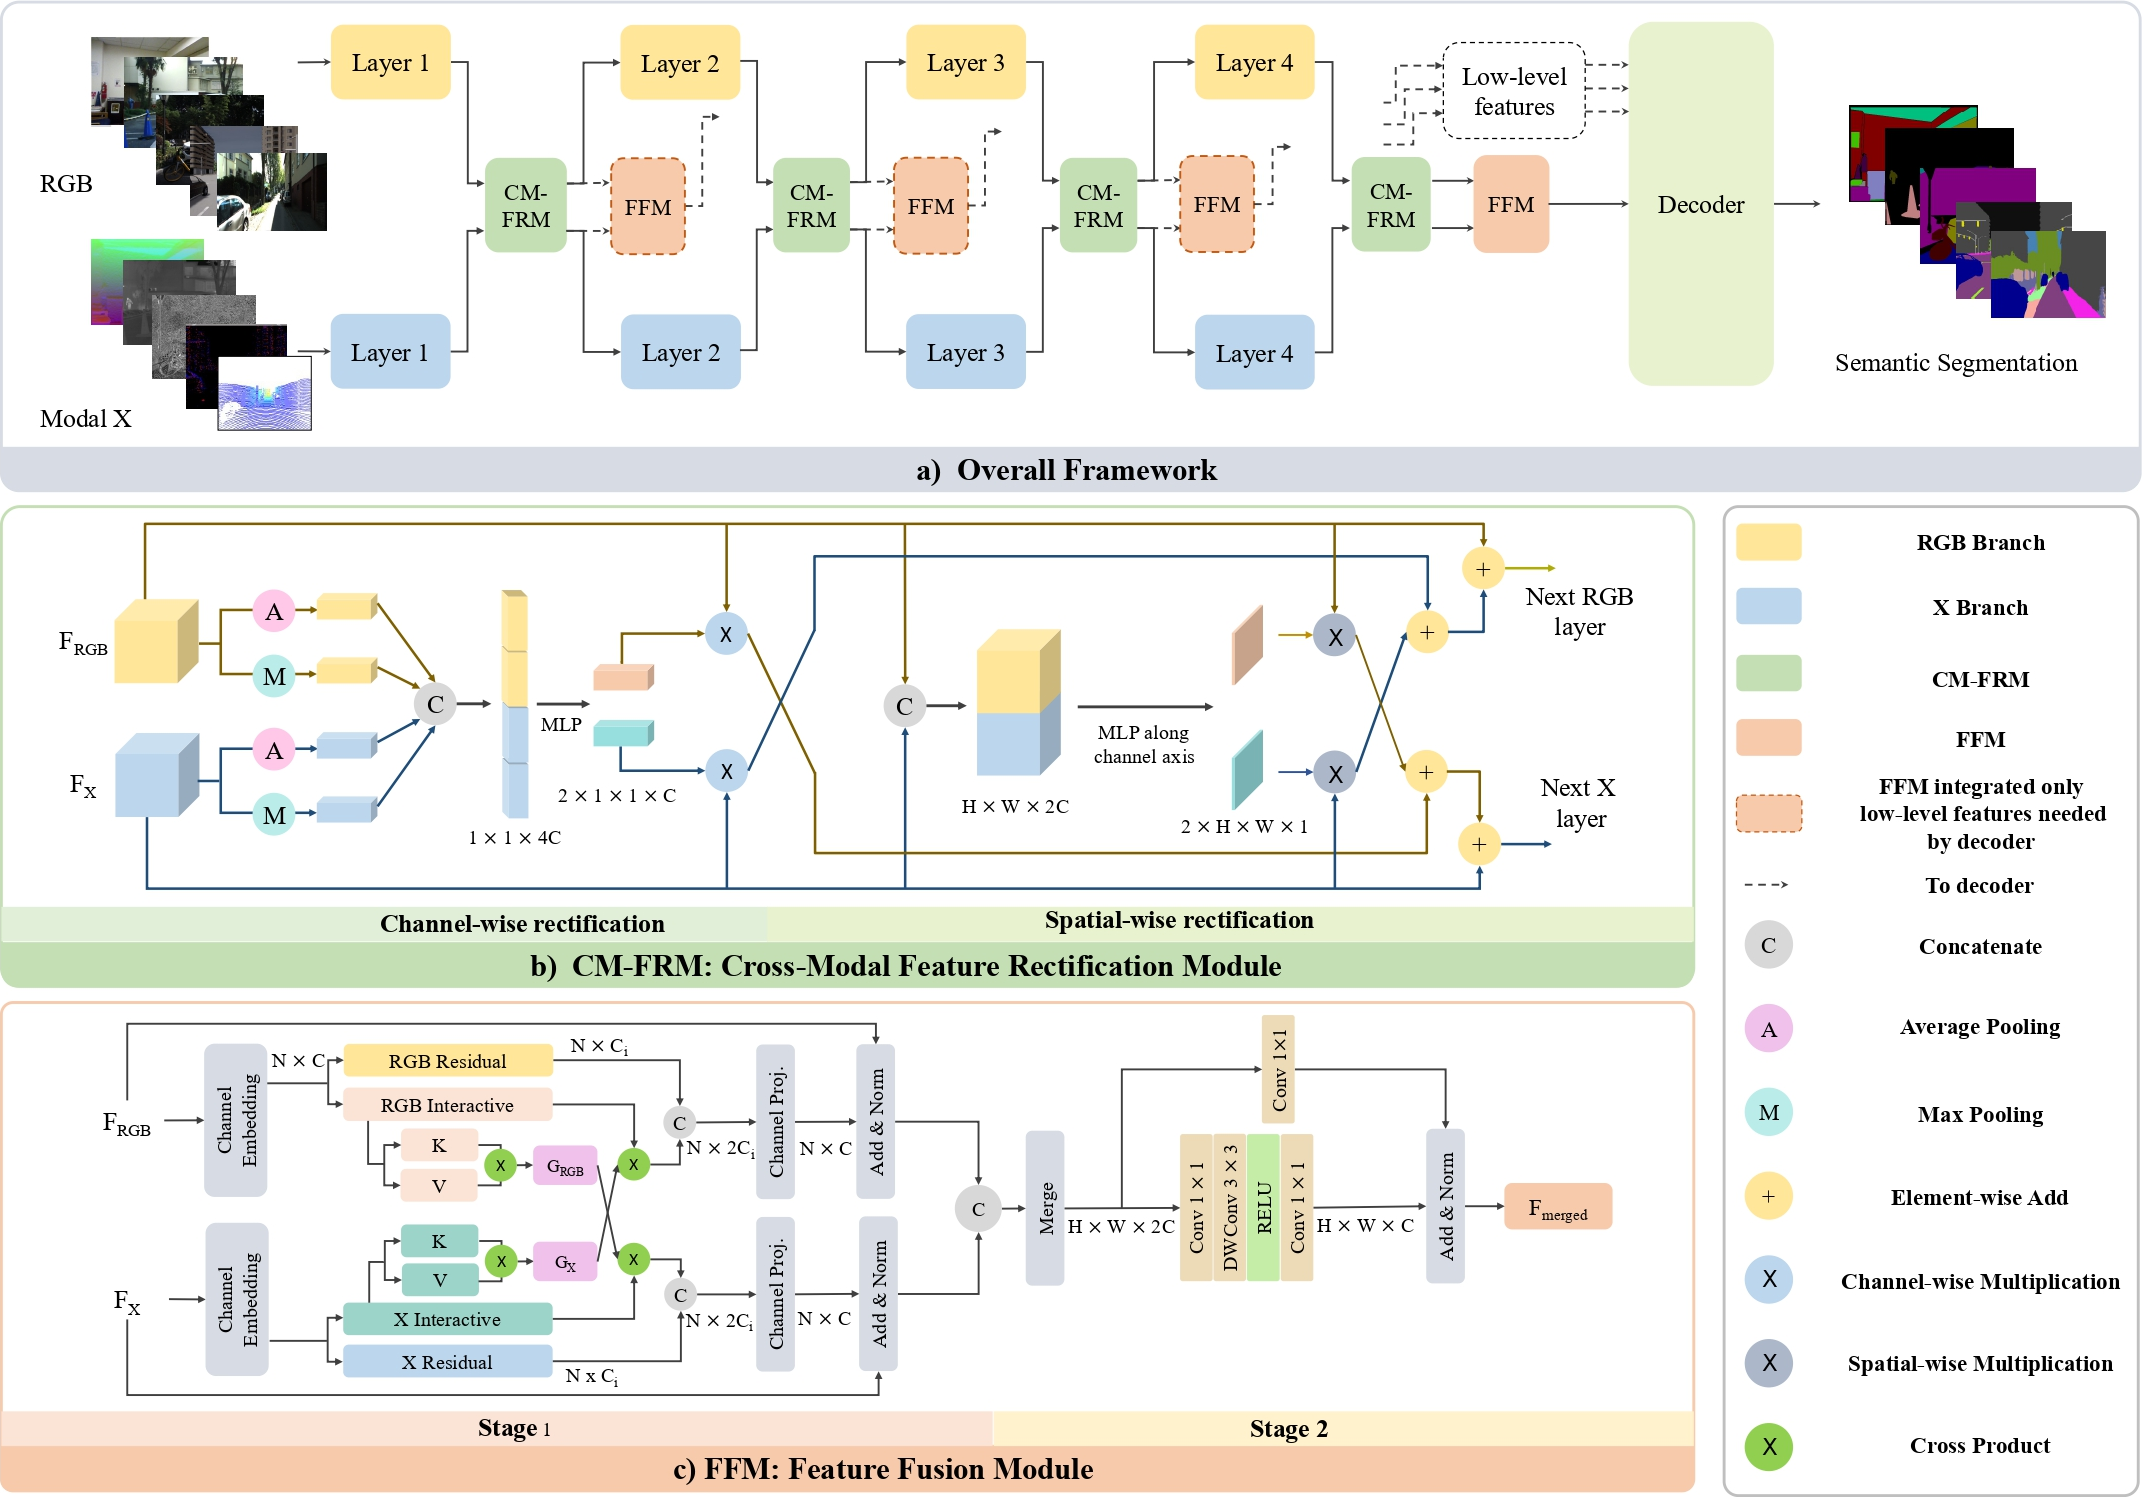
\includegraphics[width=\textwidth]{media/model/cmx_architecture.png}
    \caption{Arquitectura propuesta por \cite{zhang2023cmxcrossmodalfusionrgbx}}
    \label{fig:cmx-architecture}
\end{figure}

La arquitectura de \texttt{CMX} (figura \ref{fig:cmx-architecture}) hace uso de dos módulos clave para la interacción y fusión de características intermodales: el \textit{Cross-Modal Feature Rectification Module} (\texttt{CM-FRM}), empleado para calibrar las características bimodales aplicando una rectificación que sería capaz de mitigar ruidos y aprovechar las complementareidades entre modalidades, y el \textit{Feature Fusion Module} (\texttt{FFM}), que somete a las características a un mecanismo de atención cruzada previo a su fusión. Este método de fusión de características supera con creces otras técnicas tradicionales como la fusión de características mediante concatenación o suma ya que permite un análisis más profundo de aquello que correlaciona ambas modalidades.

Además, a pesar de que el \textit{backbone} preentrenado que se ofrece está entrenado en \texttt{ImageNet} y, por tanto, sus pesos están adaptados a \texttt{RGB-RGB}, se asegura la adaptabilidad del mismo a una gran variedad de modalidades \texttt{RGB-X} mediante \textit{transfer learning}, por lo que se espera que el modelo sea capaz de adaptarse fácilmente a las necesidades de este trabajo, siendo \texttt{IR} un buen sustituto del original \texttt{RGB} debido a la similaridad de su dominio y \texttt{D} aquella modalidad extra \texttt{D}.

\section{Técnicas de Pre-Procesado}
\label{sec:preprocessing_techniques}
Cuando vamos a usar una imagen como input para un modelo de segmentación, se debe tener en cuenta el formato en el que se desea representar la información que se le proporciona al modelo. En este caso, se cuenta con dos modalidades de entrada: \texttt{IR} y \texttt{D}, por lo que es interesante el análisis de las posibles técnicas de preprocesado que se pueden aplicar a cada modalidad para obtener un mejor resultado en la segmentación.

Así como aumentar la información que otorga el canal \texttt{IR} es una tarea complicada, ya que la imagen ya cuenta con una calidad aceptable y que dificilmente se mejorará con ninguna técnica de preprocesado (además de ser tan similar a aquellos pesos preentrenados en \texttt{ImageNet}), el canal \texttt{D} es el que más margen de operación presenta debido a la gran cantidad de ruido presene y, al contrario que con la modalidad \texttt{IR}, el que el modelo más dificultades tenga a la hora de extraer características debido a su escasa similaridad con los datos de pre-entrenamiento en \texttt{ImageNet}. Es por esto que se propone aplicar las técnicas de pre-procesado exclusivamente al canal \texttt{D} con el fin de aumentar la información disponible para el modelo e, idealmente, que este aprenda a emplear las características de forma más efectiva.

Existe una variedad de técnicas de pre-procesado que aprovechan los tres canales de entrada del modelo para así lograr un \textit{input} capaz de aportar mayor cantidad de información al modelo de segmentación. A continuación, se presentan las técnicas de pre-procesado que se proponen para este trabajo.

\subsection{HHA Encoding}
\label{subsec:hha_encoding}
Esta técnica, propuesta por \cite{gupta2014learningrichfeaturesrgbd} y siendo la técnica recomendada por los autores de \texttt{CMX} para el preprocesado de imágenes de profundidad, emplea los tres canales de la imagen de entrada para codificar las siguientes tres características:
\begin{itemize}
    \item Ángulo con respecto a la gravedad
    \item Altura sobre el suelo
    \item Disparidad horizontal
\end{itemize}
Esta colorización, además de representar características que difícilmente serían aprendidas por el modelo si no se codificaran en la imagen de entrada, aprovecha los tres canales de entrada al \textit{encoder}, por lo que más información es aportada en la entrada. A pesar de que esta colorización permite calcular las características mencionadas, es importante destacar que el cambio de dominio es mucho más radical que otras alternativas propuestas en esta sección, por lo que los pesos preentrenados en \texttt{ImageNet} no supondrán una base de entrenamiento tan robusta.

\begin{figure}[!h]
    \centering
    \begin{subfigure}{0.45\textwidth}
        \centering
        \includegraphics[width=\textwidth]{media/data/depth_gueese.png}
        \caption{Imagen de profundidad base}
        \label{fig:depth-base-hha}
    \end{subfigure}
    \hfill
    \begin{subfigure}{0.45\textwidth}
        \centering
        \includegraphics[width=\textwidth]{media/data/hha_gueese.png}
        \caption{Profundidad colorizada con \texttt{HHA}}
        \label{fig:hha-colorization}
    \end{subfigure}
    \caption{Comparación entre la imagen de profundidad base y la imagen de profundidad codificada con \texttt{HHA}}
    \label{fig:hha-comparison}
\end{figure}

Por otra parte, es importante destacar que el tiempo de cómputo necesario para realizar esta operación puede ser elevado (alrededor de 4.4 segundos en el equipo de testeo), por lo que la aplicación de esta técnica estaría limitada a casos en los que su aplicación en tiempo real no sea necesaria a no ser que se realizase una implementación extremadamente optimizada del algoritmo. Un ejemplo de esta técnica se muestra en la figura \ref{fig:hha-colorization}, donde se puede observar una gran cantidad de ruido presente en la imágen \texttt{HHA} derivado del ruido presente en la imagen de profundidad original, lo que podría suponer una dificultad para el modelo a la hora de aprender las características de la escena ya que esta técnica suele reservarse para imágenes tomadas en interior, donde la cantidad de ruido es mucho menor.

\subsection{Colorizacón Jet}
\label{subsec:jet_colorization}
En el trabajo desarrollado en \cite{eitel2015multimodaldeeplearningrobust} se propone como alternativa a \texttt{HHA} la colorización de la imagen de entrada usando el esquema de color \textit{Jet}. Esto, a pesar de no aportar información adicional sobre la imágen de profundidad original, sí que, en cierta forma, ``ordena`` la información de profundidad en los canales \texttt{RGB}, lo que implica dos posibles ventajas: la imágen resultante se asemeja mucho más a las imágenes \texttt{ImageNet} sobre las que el backbone ha sido preentrenado y, por otro lado, facilita el aprendizaje del modelo al asignar valores cromáticos distintos a profundidades diferentes, haciendo más explícitas las diferencias espaciales en la escena.

\begin{figure}[!h]
    \centering
    \begin{subfigure}{0.45\textwidth}
        \centering
        \includegraphics[width=\textwidth]{media/data/depth_gueese.png}
        \caption{Imagen de profundidad base}
        \label{fig:depth-base-jet}
    \end{subfigure}
    \hfill
    \begin{subfigure}{0.45\textwidth}
        \centering
        \includegraphics[width=\textwidth]{media/data/jet_gueese.png}
        \caption{Profundidad colorizada con \textit{Jet}}
        \label{fig:jet-colorization}
    \end{subfigure}
    \caption{Comparación entre la imagen de profundidad base y la imagen de profundidad codificada con Jet}
    \label{fig:jet-comparison}
\end{figure}

Como se puede ver en la figura \ref{fig:jet-colorization}, cada píxel es asignado con un valor \texttt{RGB} dependiendo únicamente de su valor de profundidad siguiendo una tabla de colorización estándar \textit{Jet} como la típicamente empleada en \texttt{OpenCV}. Este proceso, a pesar de no aportar información adicional como en el caso de \texttt{HHA}, es mucho más rápido y sencillo de implementar. Además, como se aprecia en la figura \ref{fig:jet-comparison}, la imagen resultante es mucho más clara y la existencia de ruido no resulta tan crítica. Como se menciona en \cite{eitel2015multimodaldeeplearningrobust}, la aplicación de este preprocesado no necesariamente supone una mejora en el rendimiento del modelo, pero sí que alcanza unos resultados muy similares a cambio de un menor tiempo de cómputo.

\subsection{Colorización por Distancia}
\label{subsec:distance_colorization}
Considerando los resultados obtenidos empleando la colorización \textit{Jet}, se propone en una técnica de colorización que, si bien puede no resultar tan visualmente atractiva para el ojo humano como su alternativa, podría codificar la distancia de forma más efectiva para el modelo. En específico, se propone establecer una relación lineal entre los valores de profundidad y el valor de los canales de la imagen final de forma que los objetos más lejanos serán más dominados por el canal \texttt{R}, mientras que los objetos más cercanos serán más dominados por el canal \texttt{B} pasando por el canal \texttt{G} en el rango intermedio. Un ejemplo de esta técnica se muestra en la figura \ref{fig:distance-colorization}.

\begin{figure}[!h]
    \centering
    \begin{subfigure}{0.45\textwidth}
        \centering
        \includegraphics[width=\textwidth]{media/data/depth_gueese.png}
        \caption{Imagen de profundidad base}
        \label{fig:depth-base-distance}
    \end{subfigure}
    \hfill
    \begin{subfigure}{0.45\textwidth}
        \centering
        \includegraphics[width=\textwidth]{media/data/depth_gueese.png}
        \caption{Profundidad colorizada por distancia}
        \label{fig:distance-colorization}
    \end{subfigure}
    \caption{Comparación entre la imagen de profundidad base y la imagen de profundidad codificada con Jet}
    \label{fig:distance-comparison}
\end{figure}

De esta manera, esta técnica es también es extremadamente rápida de aplicar al basarse en asignar un valor \texttt{RGB} a cada píxel dependiendo de su valor de intensidad. La interpolación de los valores de distancia a estos valores podría ser aprendida por el modelo de forma algo más efectiva que en el caso de Jet debido a la mayor simplifidad en su distribución, ya que no fomenta tanto una imagen placentera a la vista sino una organización en los canales \texttt{RGB} más directa.

\subsection{Normales}
\label{subsec:normals}
De nuevo, siguiendo los resultados presentados por \cite{eitel2015multimodaldeeplearningrobust}, una mejor y más rápida solución de postprocesado podría tratarse de la codificación de las normales en la imagen de entrada. Esta técnica consiste en calcular el vector normal de la superficie de cada pixel partiendo de la imagen de profundidad y codificarlo en los tres canales del \textit{input} del modelo. Para comprender cómo se realiza esta conversión es necesario entender que la imagen de profundidad es tan solo una representación de los diferentes valores de distancia de los objetos en la escena, lo que supone una conversión directa de la imagen de profundidad 2D a una nube de puntos en un espacio 3D. Esto supone que cada uno de los puntos se puede asociar con un vector normal en \texttt{XYZ} que representa la orientación de la superficie en ese punto, siendo estos vectores fácilmente codificables en los canales \texttt{RGB} de la imagen de entrada.

\begin{figure}[!h]
    \centering
    \begin{subfigure}{0.45\textwidth}
        \centering
        \includegraphics[width=\textwidth]{media/data/depth_gueese.png}
        \caption{Imagen de profundidad base}
        \label{fig:depth-base-distance}
    \end{subfigure}
    \hfill
    \begin{subfigure}{0.45\textwidth}
        \centering
        \includegraphics[width=\textwidth]{media/data/normal_gueese.png}
        \caption{Profundidad colorizada por normales}
        \label{fig:normals-colorization}
    \end{subfigure}
    \caption{Comparación entre la imagen de profundidad base y la imagen de profundidad codificada con normales}
    \label{fig:normals-comparison}
\end{figure}

De esta forma, este tipo de codificación también aporta información adicional al modelo que dificilmente se podría aprender de otra forma, como puede ser la orientación de los objetos en la escena o incluso los bordes de los mismos (en decrimento de la información de profundidad). Un ejemplo de esta técnica se muestra en la figura \ref{fig:normals-colorization} donde se puede apreciar que el método, por razones similares a las de la colorización \texttt{HHA}, presenta cierto nivel de ruido en la imagen resultante.

\begin{equation}
    \begin{aligned}
        \hat{n} = \frac{(n_x, n_y, 1)}{\sqrt{n_x^2 + n_y^2 + 1}} \\
        n_x = \frac{\partial z}{\partial x}, n_y = \frac{\partial z}{\partial y} 
    \end{aligned}
    \label{eq:normals}
\end{equation}

La imagen final se obtiene calculando las derivadas parciales respecto a $x$ e $y$ de los valores de profundidad en la modalidad \texttt{D} mediante la aplicación de un filtro \texttt{Sobel} y normalizando el vector resultante como se muestra en la ecuación \ref{eq:normals}.

\section{Entrenamiento}
\label{sec:cmx_training}
El entrenamiento del modelo es realizado en un ordenador portátil con una tarjeta gráfica \texttt{NVIDIA GeForce GTX 1650} con 4GB de memoria \texttt{VRAM} y un procesador \texttt{Intel Core i5-10300H} con 8 núcleos y 16 hilos, así como 16GB de memoria \texttt{RAM}. Además, como se ha mencionado en los anteriores apartado, se empleará un \textit{backbone} pre-entrenado en \texttt{ImageNet} y se aplicará la técnica de \textit{transfer learning} para adaptar el modelo a las características de los datos de entrada. El modelo se entrenará durante 500 épocas realizando validaciones periódicas con el objetivo de verificar el correcto aprendizaje de la red y evitar \textit{overfitting}, además de aplicar \textit{data augmentation} mediante el recorte de las imágenes originales en imágenes más pequeñas con este mismo fin de aumentar (artificialmente) los datos de entrenamiento para evitar \textit{overfitting} y fomentar el aprendizaje de características generales y no tanto de características específicas de los datos de entrenamiento.

\begin{table}[!h]
    \centering
    \begin{tabular}{|c|c|c|c|}
        \hline
        \textbf{Entrenamiento} & \textbf{IR+D} & \textbf{Depth} & \textbf{InfraRed} \\
        \hline
        Sin Modality Dropout & 73.902\% & 19.844\% & 60.597\% \\
        Con Modality Dropout & 80.907\% & 66.099\% & 80.026\% \\
        \hline
    \end{tabular}
    \caption{Comparación de la aplicación de \textit{modality dropout}}
    \label{tab:modality_dropout_comparison}
\end{table}

Por otra parte, tras observar que un entrenamiento típico puede generar que el modelo aprenda a emplear una de las modalidades de entrada de forma más efectiva que la otra, siendo esta última empleada como una suerte de "refuerzo" que tan solo amplía la información de la otra modalidad pero no es capaz de aportar la suficiente información por si misma, y dado que sería ideal que el modelo sea capaz de desenvolverse sin problema cuando, por el motivo que sea, una de las modalidades no esté disponible, se opta por aplicar \textit{modality dropout} en el entrenamiento. Esta técnica consiste en la eliminación aleatoria de una de las modalidades de entrada del modelo durante el entrenamiento. De esta forma, durante los primeros compases del entrenamiento, el modelo aprenderá a emplear las características de forma independiente en ambas modalidades, y a medida que éste avance, se fomentará el aprendizaje de las características de forma conjunta. Como se puede observar comparando las figuras (TODO y TODO) en las que se muestra las matrices de confusión para las distintas combinaciones de modalidades de entrada, el modelo tiende a aprender mucho más de la modalidad \texttt{IR} ya que es la que mayor información aporta, pero aun siendo así, gracias a la aplicación del \textit{modality dropout}, el modelo puede realizar una segmentación adecuada incluso cuando tan solo se cuenta con la modalidad \texttt{D}. Los beneficios de implementar esta técnica se pueden observar en la tabla \ref{tab:modality_dropout_comparison}, donde se ve una clara mejora en la segmentación cuando falta una de las modalidades de entrada si el entrenamiento se ha realizado con \textit{modality dropout}.

\subsection{Implementación}
\label{subsec:implementation}
Para este trabajo se implementará el backbone \textit{Mix Transformer} (\texttt{MiT}) preentrenado en \texttt{ImageNet} y basado en el \textit{framework} \texttt{SegFormer} (ambos presentados en \cite{xie2021segformersimpleefficientdesign}) en su versión más pequeña, el \texttt{MiT-B0}. Este \textit{encoder}, junto al \textit{decoder} \texttt{MLP} para segmentación, suman un total de 3.8M de parámetros entrenables. La implementación del modelo sobre el \textit{dataset} del que se cuenta se realiza adaptando el código disponible en el repositorio de \textit{GitHub} asociado al trabajo original (\cite{zhang2023cmxcrossmodalfusionrgbx}), siendo los cambios realizados los necesarios para adaptar el \textit{DataLoader} al formato \texttt{COCO} en el que se encuentran los datos de entrenamiento, la implamentación de técnicas como el \textit{Modality Dropout} y la validación durante el entrenamiento con el fin de evitar \textit{overfitting}. Además, se respeta la implementación original en \texttt{PyTorch} por simplicidad y por facilidad de uso.

La función de pérdida empleada durante el entrenamiento será \textit{CrossEntropyLoss} y el optimizador se trata de \texttt{Adam} con una tasa de aprendizaje de $10^{-6}$ dinámica con un momento de 0.9. El modelo se entrenará durante 500 épocas con un tamaño de \textit{batch} de 2 pares \texttt{IR}-\texttt{D} (de nuevo, debido a los limitados recursos con  los que se cuenta, en este caso una \texttt{GPU} con tan solo 4 GB de \texttt{VRAM}).

Además, la implementación del \textit{modality dropout} se realiza de forma que durante las primeras épocas de entrenamiento exista un 50\% de probabilidad de que una de las dos modalidades de entrenamiento esté ausente, siendo ese el caso, la modalidad \texttt{IR} faltará con una probabilidad del 65\%, mientras que la \texttt{D} (aquella cuyo aprendizaje de características se desea fomentar) lo hará con una probabilidad del 35\%. A medida que el entrenamiento avance, la probabilidad de que una de las modalidades falte disminuirá de forma lineal hasta llegar a un 0\% en la última época de entrenamiento.

\section{Comparación de Técnicas}
\label{subsec:cmx_techniques_comparison}
Las distintas técnicas anteriores presentan diferentes resultados tras su evaluación, tal y como se puede ver en la tabla \ref{tab:techniques_comparison} y en las diferentes matrices de confusión presentes en el anexo (TODO: referir al anexo!!!). En la tabla \ref{tab:techniques_comparison} se muestra la media entre las diferentes clases (\textbf{Background}, \textbf{Deer}, \textbf{Goat}, \textbf{Donkey} y \textbf{Goose}) del índice de Jaccard o \textit{Index Over Union} (\ref{eq:iou}) obtenida por cada una de las técnicas de pre-procesado propuestas para cada uno de las posibles casuísticas de ausencia o presencia de las modalidades \texttt{IR} y \texttt{D}. Aquí, se puede apreciar que la colorización \texttt{Jet} es la mejor opción cuando ambas modalidades están disponibles, aunque, por otro lado, se puede apreciar como éste no necesariamente es el caso cuando alguna de las modalidades se encuentra ausente.

\begin{table}[!h]
    \centering
    \begin{tabular}{|c|c|c|c|}
        \hline
        \textbf{Técnica} & \textbf{IR+D} & \textbf{Depth} & \textbf{InfraRed} \\
        \hline
        Sin Pre-Procesado & 80.907\% & 66.099\% & 80.026\% \\
        HHA Encoding & 80.620\% &  30.702\% &  80.293\%\\
        Colorización Jet & 81.677\% & 63.274\% & 78.230\%\\
        Colorización por Distancia & 81.422\% & 57.659\% & 79.027\%\\
        Normales & 79.566\% & 47.340\% & 78.760\%\\
        \hline
    \end{tabular}
    \caption{IoU de las técnicas de pre-procesado propuestas}
    \label{tab:techniques_comparison}
\end{table}

\begin{equation}
    \text{IoU} = \frac{\text{Área de Superposición}}{\text{Área de Unión}}
    \label{eq:iou}
\end{equation}

Además, como se puede ver en las matrices de confusión que se encuentran en el anexo (TODO: referir al anexo!!!) todas estas técnicas comparten una precisión extremadamente alta al diferenciar entre clases, siendo la confusión con el fondo la principal fuente de error en la segmentación de las imágenes. Un ejemplo del resultado de la segmentación de una imagen empleando colorización \texttt{Jet} se muestra en la figura \ref{fig:segmentation-example}.

Por último, cabe destacar cómo las técnicas \texttt{HHA} y Normales presentan peores resultados cuando solo se cuenta con la modalidad \texttt{D}. Esto se debe principalmente a la cantidad de ruido presente en las imágenes resultantes, mientras que los otros métodos presentan resultados más consistentes debido a la simplicidad de su implementación, estos son gravemente influenciables por el ruido presente en la imagen original.

\chapter{DFormer}
\label{chap:dformer}
\section{Descripción del Modelo}
\label{sec:dformer_description}
Otro modelo relevante para este trabajo es \texttt{DFormer}, presentado por \cite{yin2024dformerrethinkingrgbdrepresentation}, que propone un marco innovador respecto al estado del arte en segmentación semántica de imágenes multimodales por la implementación de un modelo ya preentrenado en pares \texttt{RGB-D} (al contrario del habitual preentreno en pares \texttt{RGB-RGB}) con la reducción de costes computacionales que esto supone. Este modelo redefine la forma en que se aprenden las características conjuntas de \texttt{RGB} y \texttt{Depth}, permitiendo mejorar el rendimiento en tareas de segmentación semántica de imágenes \texttt{RGB-D}.

\begin{figure}[!h] 
    \centering 
    \includegraphics[width=\textwidth]{media/model/dformer_architecture.png}
    \caption{Arquitectura propuesta por \cite{yin2024dformerrethinkingrgbdrepresentation}} 
    \label{fig:dformer-architecture}
\end{figure}

La arquitectura de \texttt{DFormer} (figura \ref{fig:dformer-architecture}) se basa en un ya típico esquema \textit{encoder}-\textit{decoder}, en concreto el \textit{encoder} jerárquico en varias etapas está diseñado para generar características a diferentes escalas. Cada una de estas etapas incluye una serie de bloques \texttt{RGB-D} consistentes en un módulo de atención global (\texttt{GAA}) y un modulo de mejora local (\texttt{LEA}) que potencian la localización de objetos fomentando el entendimiento 3D de la escena y que capturan información local a partir de la información de profundidad (figura \ref{fig:dformer-blocks}).

\begin{figure}[!h]
    \centering
    \includegraphics[width=0.5\textwidth]{media/model/dformer_block.png}
    \caption{Bloques \texttt{RGB-D} propuestos por \cite{yin2024dformerrethinkingrgbdrepresentation}}
    \label{fig:dformer-blocks}
\end{figure}

\section{El pre-entrenamiento}
\label{sec:dformer_pretraining}
Una importante mejora que se implementa en \cite{yin2024dformerrethinkingrgbdrepresentation} consiste en el preentrenamiento en pares \texttt{RGB-D}. Estos pares son conseguidos aplicando técnicas de estimación de la profundidad sobre los datos presentes en \texttt{ImageNet}, lo que permite el pre-entrenamiento del modelo en un gran conjunto de datos ya estandarizado sin necesidad de recurrir al etiquedado de pares \texttt{RGB-D} o a datasets de menor tamaño. Este pre-entrenamiento en pares \texttt{RGB-D} estimados permitirá al modelo aprender a emplear y combinar las características de ambas modalidades de forma más efectiva de cara al \textit{transfer learning} sobre el que ya se contará con un \textit{prior} de calidad, lo que es una ventaja sobre otros modelos preentrenados en pares \texttt{RGB-RGB} que deben aprender el cambio de dominio durante el entrenamiento final.

\section{Resultados}
\label{sec:dformer_results}
El entrenamiento de este modelo es mucho más directo que en el caso de \texttt{CMX} ya que no se requiere de ningún tipo de preprocesado de la modalidad de profundidad para acercarla a la modalidad \texttt{RGB} original, por lo que se puede emplear directamente el canal \texttt{D} original sin la necesidad de alterarlo de ningún modo. Sin embargo, TODO: POR Q NO FUNCIONA??????

\chapter{Resultados}
\label{chap:results}
\section{Cross Modal Fusion}
\label{sec:cmx_results}
Empleando el modelo \texttt{SegFormer} presentado en \cite{strudel2021segmentertransformersemanticsegmentation} como punto de comparación para el desempeño de \texttt{CMX} (ya que este último se construye sobre el primero), se puede observar que el uso de técnicas multimodales supone una gran mejora en los resultados de segmentación, siendo el caso de mejor desempeño aquel en el que se aplica un preprocesado mediante colorización \textit{Jet}, en la tabla \ref{tab:segformer_cmx_comparison} se puede ver como claramente el empleo de dos modalidades aumenta la calidad de las características aprendidas por el modelo, lo que deriva en una segmentación más precisa.

\begin{table}[!h]
    \centering
    \begin{tabular}{|c|c|}
        \hline
        \textbf{Modelo} & \textbf{\texttt{IoU} medio} \\
        \hline
        SegFormer & 66.894\% \\
        CMX (\texttt{IR-IR}) & 73.770\% \\
        CMX (\texttt{IR-D}) & 81.677\% \\
        \hline
    \end{tabular}
    \caption{Comparación de los resultados de segmentación entre un modelo \texttt{SegFormer} básico, \texttt{CMX} entrenado tan solo en la modalidad \texttt{IR} y \texttt{CMX} entrenado en pares \texttt{IR-D}}
    \label{tab:segformer_cmx_comparison}
\end{table}

Así mismo, también cabe destacar que entrenando el modelo \texttt{CMX} en pares duplicados \texttt{IR-IR} (la misma imagen en ambas entradas) se desarrolla la tarea de segmentación mucho mejor que el modelo \texttt{SegFormer} a pesar de estar basados en la misma arquitectura. Esto se debe a que, además de que el modelo \texttt{CMX} resultaría ser mas grande al tener dos \textit{encoders} en paralelo, éste extrae características de la entrada duplicada de forma simultánea para más tarde fusionarlas de forma inteligente, lo que, a pesar de contar con la misma información en ambas entradas, permite al modelo comprender mejor la escena. Siendo este el caso, no sería justa una comparación directa entre \texttt{SegFormer} y \texttt{CMX} multimodal dada la naturaleza más avanzada del segundo, por lo que únicamente se puede concluir la utilidad de la multimodalidad en la segmentación de imágenes si comparamos los resultados de \texttt{CMX} en pares \texttt{IR-D} con los de \texttt{CMX} en pares duplicados \texttt{IR-IR}, caso en el que se aprecia una gran mejora de la segmentación cuando existen diferentes modalidades a la entrada del modelo, verificando así la hipótesis inicial.

\begin{figure}
    \begin{subfigure}{0.45\textwidth}
        \centering
        \includegraphics[width=\textwidth]{media/data/cmx_output.png}
        \caption{Output del modelo}
    \end{subfigure}
    \hfill
    \begin{subfigure}{0.45\textwidth}
        \centering
        \includegraphics[width=\textwidth]{media/data/gueese_gt.png}
        \caption{Ground Truth}
    \end{subfigure}
    \caption{Resultados de la segmentación}
    \label{fig:segmentation-example}
\end{figure}

% \chapter{Seguimiento de los animales}
% \label{chap:tracking}
% TODO: implementación del seguimiento de los animales con abewley/SORT

\chapter{Conclusiones y trabajo futuro}

\section{Conclusiones}
En este trabajo, se ha explorado la aplicación de técnicas de segmentación multimodal en el ámbito con el fin de demostrar su eficacia en posibles aplicaciones de ciber-pastoreo. Se implementaron y evaluaron dos modelos principales: \textit{Cross Modal Fusion (CMX)} y \textit{DFormer}, ambos diseñados para aprovechar la información complementaria de las imágenes infrarrojas (IR) y de profundidad (D). Además, se evaluaron distintas técnicas de preprocesado para el primero de los casos, pretendiendo encontrar formas de adaptar métodos no específicos a esta modalidad, como la colorización de imágenes de profundidad o la codificación de otro tipo de características matemáticas extraíbles de la misma.

Los resultados obtenidos demuestran que la combinación de modalidades IR y D permite una segmentación más precisa y robusta en comparación con el uso de modalidades individuales. Entre las técnicas evaluadas, \texttt{CMX} con preprocesado mediante colorización \textit{Jet} se destacó como una solución eficiente y de bajo costo computacional capaz de rendir mejor que sus alternativas, especialmente en escenarios donde ambas modalidades están disponibles. Por otro lado, la aplicación de \textit{modality dropout} durante el entrenamiento resultó ser fundamental para aumentar la robustez del modelo ante la ausencia de una de las modalidades.

Aunque los resultados son prometedores, se identificaron algunas limitaciones, como la sensibilidad del modelo al ruido presente en las imágenes de profundidad dado a la naturaleza del sensor y el entorno en el que se desarrolla la acción. Estas limitaciones abren la puerta a nuevas líneas de investigación que se describen a continuación.

\section{Trabajo futuro}
A partir de las conclusiones extraídas de este trabajo, se plantean las siguientes líneas de investigación para mejorar y expandir los resultados obtenidos:

\begin{itemize}
    \item \textbf{Optimización del preprocesado:} Investigar nuevas técnicas de preprocesado que reduzcan el ruido en las imágenes de profundidad, paralelización el procesado de imágenes para posibles apicaciones en tiempo real, algoritmos de filtrado avanzado o técnicas de aprendizaje profundo específicas para la limpieza de datos.

    \item \textbf{Ampliación del dataset:} Utilizar datasets más diversos y extensos que incluyan diferentes tipos de animales, entornos y condiciones de iluminación, con el objetivo de mejorar la capacidad de generalización de los modelos. Posible inclusión de datos sintéticos como se hace en \cite{haucke2021exploitingdepthinformationwildlife}.

    \item \textbf{Implementación en tiempo real:} Adaptar los modelos para aplicaciones en tiempo real mediante la optimización de los algoritmos mediante \textit{frameworks} como \texttt{TensorRT} o \texttt{ONNX} y el uso de hardware especializado, como cámaras integradas con capacidades de procesamiento local.

    \item \textbf{Fusionar modalidades adicionales:} Integrar otras modalidades, como datos infrarojos térmicos o cámaras de eventos, para enriquecer la información de entrada y mejorar la precisión en escenarios más complejos.

    \item \textbf{Evaluación en entornos reales:} Validar el desempeño de los modelos en situaciones reales de ciber-pastoreo, analizando su efectividad y adaptabilidad en aplicaciones prácticas.
    
    \item \textbf{Aplicación en imágen aérea:} Aplicación de las técnicas en imágenes aéreas para un seguimiento más amplio y cercano a un escenario real de ciber-pastoreo.
\end{itemize}

En resumen, este trabajo establece una base sólida para la aplicación de la segmentación multimodal en el ciber-pastoreo y abre nuevas oportunidades para la investigación y desarrollo de sistemas más robustos y eficientes en este campo.


\appendix
\label{app:appendix_a}
% TODO: whatever appendices :)

\bibliography{refs.bib}
\bibliographystyle{IEEEtran}

\end{document}